\documentclass[12pt]{article}

\usepackage{amsmath, mathtools}
\usepackage{amsfonts}
\usepackage{amssymb}
\usepackage{graphicx}
\usepackage{colortbl}
\usepackage{xr}
\usepackage{hyperref}
\usepackage{longtable}
\usepackage{xfrac}
\usepackage{tabularx}
\usepackage{float}
\usepackage{siunitx}
\usepackage{booktabs}
\usepackage{caption}
\usepackage{pdflscape}
\usepackage{afterpage}
\usepackage{tikz}

\usepackage[round]{natbib}

%\usepackage{refcheck}

\hypersetup{
    bookmarks=true,         % show bookmarks bar?
      colorlinks=true,       % false: boxed links; true: colored links
    linkcolor=red,          % color of internal links (change box color with linkbordercolor)
    citecolor=green,        % color of links to bibliography
    filecolor=magenta,      % color of file links
    urlcolor=cyan           % color of external links
}

%%% Comments

\usepackage{color}

\newif\ifcomments\commentstrue

\ifcomments
\newcommand{\authornote}[3]{\textcolor{#1}{[#3 ---#2]}}
\newcommand{\todo}[1]{\textcolor{red}{[TODO: #1]}}
\else
\newcommand{\authornote}[3]{}
\newcommand{\todo}[1]{}
\fi

\newcommand{\wss}[1]{\authornote{blue}{SS}{#1}}
\newcommand{\an}[1]{\authornote{magenta}{Author}{#1}}


% For easy change of table widths
\newcommand{\colZwidth}{1.0\textwidth}
\newcommand{\colAwidth}{0.13\textwidth}
\newcommand{\colBwidth}{0.82\textwidth}
\newcommand{\colCwidth}{0.1\textwidth}
\newcommand{\colDwidth}{0.05\textwidth}
\newcommand{\colEwidth}{0.8\textwidth}
\newcommand{\colFwidth}{0.17\textwidth}
\newcommand{\colGwidth}{0.5\textwidth}
\newcommand{\colHwidth}{0.28\textwidth}

% Used so that cross-references have a meaningful prefix
\newcounter{defnum} %Definition Number
\newcommand{\dthedefnum}{GD\thedefnum}
\newcommand{\dref}[1]{GD\ref{#1}}
\newcounter{datadefnum} %Datadefinition Number
\newcommand{\ddthedatadefnum}{DD\thedatadefnum}
\newcommand{\ddref}[1]{DD\ref{#1}}
\newcounter{theorynum} %Theory Number
\newcommand{\tthetheorynum}{T\thetheorynum}
\newcommand{\tref}[1]{T\ref{#1}}
\newcounter{tablenum} %Table Number
\newcommand{\tbthetablenum}{T\thetablenum}
\newcommand{\tbref}[1]{TB\ref{#1}}
\newcounter{assumpnum} %Assumption Number
\newcommand{\atheassumpnum}{P\theassumpnum}
\newcommand{\aref}[1]{A\ref{#1}}
\newcounter{goalnum} %Goal Number
\newcommand{\gthegoalnum}{P\thegoalnum}
\newcommand{\gsref}[1]{GS\ref{#1}}
\newcounter{instnum} %Instance Number
\newcommand{\itheinstnum}{IM\theinstnum}
\newcommand{\iref}[1]{IM\ref{#1}}
\newcounter{reqnum} %Requirement Number
\newcommand{\rthereqnum}{P\thereqnum}
\newcommand{\rref}[1]{R\ref{#1}}
\newcounter{lcnum} %Likely change number
\newcommand{\lthelcnum}{LC\thelcnum}
\newcommand{\lcref}[1]{LC\ref{#1}}
\newcounter{calcnum} %Calculation Number
\newcommand{\cthecalcnum}{C\thecalcnum}
\newcommand{\cref}[1]{C\ref{#1}}
\newcounter{outputnum} %Output Number
\newcommand{\otheoutputnum}{O\theoutputnum}
\newcommand{\oref}[1]{O\ref{#1}}
\newcounter{bibnum} %Output Number
\newcommand{\bthebibnum}{\thebibnum}
\newcommand{\bref}[1]{\ref{#1}}
\newcounter{nfrnum} %NFR Number
\newcommand{\nfrthenfrnum}{\thenfrnum}
\newcommand{\nfrrref}[1]{NFR\ref{#1}}


\newcommand{\progname}{Linear Algebraic Equation Solver} % PUT YOUR PROGRAM NAME HERE

\usepackage{fullpage}

\begin{document}

\title{Commonality Analysis for a Library of Linear Algebraic Equation Solver } 
\author{Devi Prasad Reddy Guttapati}
\date{October 4, 2017}


	
\maketitle
\pagebreak
\pagenumbering{roman}
\tableofcontents

\begin{table}[bp]
\caption{\bf Revision History}
\begin{tabularx}{\textwidth}{p{3cm}p{2cm}X}
\toprule {\bf Date} & {\bf Version} & {\bf Notes}\\
\midrule
October 4, 2017 & 1.0 & Initial Draft\\

\bottomrule
\end{tabularx}
\end{table}

\section{Reference Material}



\subsection{Table of Units}

This section does not apply to this program family.

\subsection{Table of Symbols}

The table that follows summarizes the symbols used in this document along with
their units.  The choice of symbols was made to be consistent with the heat
transfer literature and with existing documentation for solar water heating
systems.  The symbols are listed in alphabetical order.

\renewcommand{\arraystretch}{1.2}
%\noindent \begin{tabularx}{1.0\textwidth}{l l X}
\noindent \begin{longtable*}{l l p{12cm}} \toprule
\textbf{symbol} & \textbf{unit} & \textbf{description}\\
\midrule


$A$ & \text{-} & known $m \times n$ matrix \\
$x$ & \text{-} & $n$-vector\\
$b$ & \text{-} & $m$-vector\\
$M_1$ & \text{-} & elementary elimination matrix\\
$L$ & \text{-} & lower triangular matrix\\
$U$ & \text{-} & upper triangular matrix\\ 
$A^{-1}$ & \text{-} & inverse of matrix \\
$I$ & \text{-} & identity matrix\\
${|A|}$ & \text{-} & determinant of matrix\\ 

\bottomrule
\end{longtable*}


\subsection{Abbreviations and Acronyms}

\renewcommand{\arraystretch}{1.2}
\begin{tabular}{l l} 
  \toprule		
  \textbf{symbol} & \textbf{description}\\
  \midrule 
  A & Assumption\\
  DD & Data Definition\\
  GD & General Definition\\
  GS & Goal Statement\\
  IM & Instance Model\\
  LC & Likely Change\\
  PS & Physical System Description\\
  R & Requirement\\
  SRS & Software Requirements Specification\\

  T & Theoretical Model\\
  O & Output\\
  \bottomrule
\end{tabular}\\



\newpage
\pagenumbering{arabic}

\section{Introduction}

Many of the relationships in nature are linear, that means their effects are
proportional to their causes. For example in Mechanics if we take Newtons second
law of motion, \textbf{$F = ma$} says that force is proportional to acceleration
and mass is the proportionality constant. For example in Electricity if we take
Ohm's Law, \textbf{$V = iR$} voltage across the conductor is proportional to the
current flowing though it and resistance is the proportionality constant. These
examples shows us the importance of linear equations and solving them. In matrix
notation the general form of linear equation is

 \centerline{\textbf{$Ax = b$}}

where \textbf{$A$} is known \textit{$m \times n$} matrix, \textbf{$b$} is an
\textit{m}-vector and \textbf{$x$} is an \textit{n}-vector. If \textbf{$x$} is
known, then such a linear relationship enables us to predict effect \textbf{$b$}
from cause \textbf{$x$} by matrix-vector multiplication \textbf{$b$} =
\textbf{$A$}\textbf{$x$}.

The most important problem in technical computing is the solution of system
linear equations.



\subsection{Purpose of Document}

The purpose of the document is to describe the methods and process for solving
the family of linear algebraic equations. A study on the method for solution of
system of linear equations and the problems effecting the effectiveness and
efficiency will be detected and correct recommendations will be made. The
significance of this document is to make a solution technique for solving family
of linear equations easier and to reduce stress on the human brain associated
with lots of reasoning when solving linear equation.

This document also describes General System Description, Commonalities,
Variabilities.

\subsection{Scope of the Family} 

The scope of the family is limited to the library of linear algebraic equation
solvers. If the user gives proper input the linear algebraic equation solver
aims to solve the equations and give the correct output.

\subsection{Characteristics of Intended Reader} 

The intended readers who read this document, must have basic knowledge about
linear algebraic equations and the different methods of solving linear algebraic
equations, which are typically covered in first and second year Linear Algebra courses .


\subsection{Organization of Document}

The template for Commonality Analysis for scientific computing software is
proposed by~\cite{smith2006systematic}. The document is organized perfectly step
by step right from the introduction to the appendix by explaining the important
concepts like General System Description, Commonalities, Variabilities.

\section{General System Description}

This section identifies the interfaces between the system and its environment,
describes the user characteristics and lists the system constraints.

\subsection{System Context}

\begin{figure}[h]
\centering
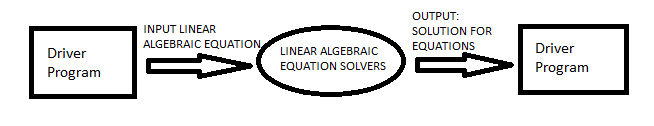
\includegraphics[scale= .7]{diagram1}
\caption{System Context}
\end{figure}



The figure shows the system context. The user gives the input in the form of
linear equations to the solver and the solver aims to give the solution to the
equations as the output.



\begin{itemize}
\item User Responsibilities:
\begin{itemize}
\item The main responsibility of the user is to give the appropriate input.
\item User must make sure that the input given is error free.
\item User must declare the method by which the linear system must be solved.
\end{itemize}
\item \progname{} Responsibilities:
\begin{itemize}
\item The main responsibility of the linear algebraic equation solver is to
identify the input which is improper or invalid.
\item Detect data type mismatch, such as a string of characters instead of a
  floating point number.
\item the ultimate responsibility of the linear algebraic equation solver is to
solve the equations and to produce the output.
\end{itemize}
\end{itemize}

\subsection{User Characteristics} \label{SecUserCharacteristics}

The end user of \progname{} should have an understanding of undergraduate Level
of Linear algebra 1 .

\subsection{System Constraints}

There are no system constraints applicable.

\section{Commonalities}

This section first presents the problem description, which gives a high-level
view of the problem to be solved. This is followed by the Terminology and
Definitions, Data Definitions, Goal Statements and Theoretical Models.

\subsection{Problem Description} \label{Sec_pd}

\progname{} is a software library which is developed to solve linear algebraic equations using numerical methods for linear algebraic equation . This solver is used to solve the linear algebraic equations with different number of variables. As many relationships in nature are linear, it will be very handy for
students to solve linear algebraic equations.

\subsection{Terminology and  Definitions}

This subsection provides a list of terms that are used in the subsequent
sections and their meaning, with the purpose of reducing ambiguity and making it
easier to correctly understand the requirements:




\begin{itemize}


\item \textbf{$A^{-1}$} is the inverse of the matrix \textbf{$A$}

\item rank(\textbf{$A$}) = The rank of a matrix is the maximum number
of linearly independent rows or columns it contains.

\item det(\textbf{$A$}) is determinant of matrix \textbf{$A$}

\item square matrix = A matrix is said to be a square matrix if and only if it has the same number of rows and columns.

\item singular matrix = A square matrix is said to be a singular matrix if it's determinant is "0".

\item upper triangular matrix = A square matrix is said to be upper triangular matrix if and only if all the entries below the main diagonal are zero.

\item lower triangular matrix = A square matrix is said to be lower triangular matrix if and only if all the entries above the main diagonal are zero.


\end{itemize}

\pagebreak

\subsection{Data Definitions} \label{sec_datadef}

~\newline

\noindent
\begin{minipage}{\textwidth}
\renewcommand*{\arraystretch}{1.5}
\begin{tabular}{| p{\colAwidth} | p{\colBwidth}|}
\hline
\rowcolor[gray]{0.9}
Number& DD\refstepcounter{datadefnum}\thedatadefnum \label{D_matrix}\\
\hline
Label& \bf Matrix Representation of the Linear Algebraic Equation\\
\hline
Symbol & \textbf{$Ax = b$}\\
\hline

  Equation&\[
\left\{ 
\begin{array}{c}
a_{11}x_1 + a_{12}x_2 + a_{13}x_3 + ........ + a_{1m}x_m = b_1 \\ 
a_{21}x_1 + a_{22}x_2 + a_{23}x_3 + ........ + a_{2m}x_m = b_2 \\
\hspace{.4cm}\vdots \hspace{1.3cm}\vdots \hspace{1.2cm}\vdots \hspace{2.6cm}\vdots \hspace{1.5cm}\vdots \\
a_{n1}x_1 + a_{n2}x_2 + a_{n3}x_3 + ........ + a_{nm}x_m = b_n \\
\end{array}
\right. 
\]\\
  \hline
  Description 
        &\textbf{$A$} is a known \textit{m x n} matrix that is 
$\begin{bmatrix}
  a_{11} & a_{12} & a_{13} & \dots & a_{1m}\\
  a_{21} & a_{22} & a_{23} & \dots & a_{2m}\\
  \vdots & \vdots & \ddots & &\vdots\\
   \vdots & \vdots &  & \ddots &\vdots\\
   a_{n1} & a_{n2} & a_{n3} & \dots & a_{nm}
   
\end{bmatrix}$.\\
        & \textbf{$b$} is an \textit{m}-vector that is
$\begin{bmatrix}
  b_1\\
  b_2\\
  \vdots\\
  b_n
\end{bmatrix}$.\\
        &\textbf{$x$} is an \textit{n}-vector that is 
$\begin{bmatrix}
  x_1\\
  x_2\\
  \vdots\\
  x_m
\end{bmatrix}$.\\
  \hline
  Source&
      \cite{heath2002scientific}
  \\
  \hline
  Ref.\ By & [\iref{gaussian}], [\iref{gauss}], [\tref{T_LAE}], [\aref{A_square}] \\
  \hline
\end{tabular}
\end{minipage}\\


~\newline

\noindent
\begin{minipage}{\textwidth}
\renewcommand*{\arraystretch}{1.5}
\begin{tabular}{| p{\colAwidth} | p{\colBwidth}|}
\hline
\rowcolor[gray]{0.9}
Number& DD\refstepcounter{datadefnum}\thedatadefnum \label{D_identity}\\
\hline
Label& \bf Identity Matrix\\
\hline
Symbol & \textbf{$I$}\\
\hline

  Equation&
\textbf{$A$}\textbf{$I$} = \textbf{$I$}\textbf{$A$} = \textbf{$A$}\\
  \hline
  Description 
        &\textbf{$A$} is a known \textit{n x n} matrix.\\

        &\textbf{$I$} is an Identity matrix .\\
        
        & $I_1$ = $\begin{bmatrix}
  1\\
\end{bmatrix}$, $I_2$ = $\begin{bmatrix}
  1 & 0\\
  0 & 1\\
\end{bmatrix}$, $I_3$ = $\begin{bmatrix}
  1, 0, 0\\
  0, 1, 0\\
  0, 0, 1\\
\end{bmatrix}$, $I_n$ = $\begin{bmatrix}
  1 & 0 & 0 & \dots & 0\\
  0 & 1 & 0 & \dots & 0\\
  0 & 0 & 1 & \dots & 0\\
  \vdots & \vdots & \vdots & \ddots &\vdots\\
  0 & 0 & 0 & \dots & 1
   
\end{bmatrix}$.\\

 \hline
  Source&
      \url{https://www.colorado.edu/engineering/Aerospace/CAS/courses.d/IFEM.d/IFEM.AppD.d/IFEM.AppD.pdf}
  \\
  \hline
  Ref.\ By & [\iref{gaussian}], [\iref{gauss}],  [\ddref{D_inverse}], [\aref{A_singular}]  \\
  \hline
\end{tabular}
\end{minipage}\\

~\newline



\noindent
\begin{minipage}{\textwidth}
\renewcommand*{\arraystretch}{1.5}
\begin{tabular}{| p{\colAwidth} | p{\colBwidth}|}
\hline
\rowcolor[gray]{0.9}
Number& DD\refstepcounter{datadefnum}\thedatadefnum \label{D_inverse}\\
\hline
Label& \bf Inverse of a Matrix\\
\hline
Symbol & \textbf{$A^{-1}$}\\
\hline

  Equation&
\textbf{$A$}\textbf{$A^{-1}$} = \textbf{$A^{-1}$}\textbf{$A$} = \textbf{$I$}\\
  \hline
  Description 
        &\textbf{$A$} is a known \textit{m x n} matrix.\\


        & \textbf{$A^{-1}$} is the inverse of matrix \textbf{$A$} .\\
        &\textbf{$I$} is an Identity matrix .\\
  \hline
  Source&
        \url{https://www.colorado.edu/engineering/Aerospace/CAS/courses.d/IFEM.d/IFEM.AppD.d/IFEM.AppD.pdf}
  \\
  \hline
  Ref.\ By & [\iref{gaussian}], [\iref{gauss}],  [\ddref{D_determinant}],  [\tref{T_LAE}], [\aref{A_singular}] \\
  \hline
\end{tabular}
\end{minipage}\\

~\newline


\noindent
\begin{minipage}{\textwidth}
\renewcommand*{\arraystretch}{1.5}
\begin{tabular}{| p{\colAwidth} | p{\colBwidth}|}
\hline
\rowcolor[gray]{0.9}
Number& DD\refstepcounter{datadefnum}\thedatadefnum \label{D_determinant}\\
\hline
Label& \bf Determinant of a Matrix\\
\hline
Symbol & \textbf{${|A|}$}\\
\hline

  Equation&
 \textbf{$${|A|} = \sum_{i=1}^{k} a_{ij} C_{ij}$$}\\
  \hline
  Description 
        &\textbf{${|A|}$} is the determinant of matrix \textbf{A}.\\


        & \textbf{ C$_{ij}$} is the cofactor of {a$_{ij}$} defined by {C$_{ij}$} = {(-1)$^{i+j}$}{M$_{ij}$} .\\

        & {M$_{ij}$} is the minor of matrix A formed by eliminating row i and column j from A.\\
        
  \hline
  Source&
       \url{http://mathworld.wolfram.com/Determinant.html}\\
       

  \hline
  Ref.\ By & [\iref{gaussian}], [\iref{gauss}],  [\ddref{D_inverse}],  [\tref{T_LAE}],  [\aref{A_singular}] \\
  \hline
\end{tabular}
\end{minipage}\\


~\newline

\noindent
\begin{minipage}{\textwidth}
\renewcommand*{\arraystretch}{1.5}
\begin{tabular}{| p{\colAwidth} | p{\colBwidth}|}
\hline
\rowcolor[gray]{0.9}
Number& DD\refstepcounter{datadefnum}\thedatadefnum \label{D_rank}\\
\hline
Label& \bf Rank of a Matrix\\
\hline
Symbol & \textbf{rank(A)}\\
\hline

  Equation&
 \textbf{rank(A) $\leq min(m, n)$}\\
  \hline
  Description 
        & rank(A) is the rank of matrix A.\\


        & The rank of a matrix can be defined as the maximum number of linearly independent column vectors in the matrix or the maximum number of linearly independent row vectors in the matrix  .\\

        & The rank of an m $\times$ n matrix is a nonnegative integer and cannot be greater than either m or n .\\
        
  \hline
  Source&
       \url{https://www.cliffsnotes.com/study-guides/algebra/linear-algebra/real-euclidean-vector-spaces/the-rank-of-a-matrix}\\
       

  \hline
  Ref.\ By & [\iref{gaussian}], [\iref{gauss}],  [\tref{T_LAE}],  \\
  \hline
\end{tabular}
\end{minipage}\\

\noindent
\begin{minipage}{\textwidth}
\renewcommand*{\arraystretch}{1.5}
\begin{tabular}{| p{\colAwidth} | p{\colBwidth}|}
\hline
\rowcolor[gray]{0.9}
Number& DD\refstepcounter{datadefnum}\thedatadefnum \label{D_utm}\\
\hline
Label& \bf Upper Triangular Matrix\\
\hline
Symbol & \textbf{$U$}\\
\hline

  Equation&
$\begin{bmatrix}
  u_{1,1} & u_{1,2} & u_{1,3} & \dots & u_{1,n}\\
         & u_{2,2} & u_{2,3} & \dots & u_{2,n}\\
                 & & \ddots & \ddots & \vdots\\
    &  &  & \ddots & u_{n-1,n}\\
   0 & & &  & u_{n,n}
   
\end{bmatrix}$.\\
  \hline
  Description 
        &\textbf{$U$} is a upper triangular matrix matrix.\\


        & A square matrix is said to be upper triangular matrix if all the entries below the main diagonal are Zero .\\
        &The sum and product of two upper triangular matrices is always a upper triangular matrix. \\
  \hline
  Source&
        \url{http://mathworld.wolfram.com/UpperTriangularMatrix.html}
  \\
  \hline
  Ref.\ By & [\iref{gaussian}], [\iref{gauss}],  [\tref{T_REF}],  [\tref{T_RREF}],  \\
  \hline
\end{tabular}
\end{minipage}\\

~\newline


\noindent
\begin{minipage}{\textwidth}
\renewcommand*{\arraystretch}{1.5}
\begin{tabular}{| p{\colAwidth} | p{\colBwidth}|}
\hline
\rowcolor[gray]{0.9}
Number& DD\refstepcounter{datadefnum}\thedatadefnum \label{D_ltm}\\
\hline
Label& \bf Lower Triangular Matrix\\
\hline
Symbol & \textbf{$L$}\\
\hline

  Equation&
$\begin{bmatrix}
  l_{1,1} &  &  &  & 0\\
  l_{2,1} & l_{2,2} &  & & \\
  l_{3,1 }& l_{3,2} & \ddots & &  \\
   \vdots & \vdots & \ddots & \ddots & \\
   l_{n,1} & l_{n,2} & \dots & l_{n,n-1} & l_{n,n}
   
\end{bmatrix}$.\\\\
  \hline
  Description 
        &\textbf{$L$} is a lower triangular matrix.\\


        & A square matrix is said to be a lower triangular matrix if all the entries above the main diagonal are zero.\\
       
  \hline
  Source&
       \url{http://mathworld.wolfram.com/LowerTriangularMatrix.html}
  \\
  \hline
  Ref.\ By & [\iref{gaussian}], [\iref{gauss}],  [\tref{T_REF}],  [\tref{T_RREF}] \\
  \hline
\end{tabular}
\end{minipage}\\

~\newline




% \begin{figure}[h!]
% \begin{center}
% %\rotatebox{-90}
% {
%  \includegraphics[width=0.5\textwidth]{<FigureName>}
% }
% \caption{\label{<Label>} <Caption>}
% \end{center}
% \end{figure}

\subsection{Goal Statements}



\begin{itemize}

\item[GS\refstepcounter{goalnum}\thegoalnum \label{G_solveforx}:] {
Given the general linear algebraic equation problem which is represented by
\textbf{Ax = b}. The initial values are A and B. The input which are the coefficients, are entered in a matrix form. If the vector b of effects is known then it would likely able to determine the corresponding vector x of cause.}

%\item[GS\refstepcounter{goalnum}\thegoalnum \label{G_InputOutput}:]{
%The user must provide the required input there by calling the linear algebraic equation solver, and the solver must display the output.}
\end{itemize}




\subsection{Theoretical Models}\label{sec_theoretical}

This section focuses on the general equations and laws that \progname{} is based
on.  

~\newline

\noindent
\begin{minipage}{\textwidth}
\renewcommand*{\arraystretch}{1.5}
\begin{tabular}{| p{\colAwidth} | p{\colBwidth}|}
  \hline
  \rowcolor[gray]{0.9}
  Number& T\refstepcounter{theorynum}\thetheorynum \label{T_LAE}\\
  \hline
  Label&\bf General Linear Algebraic Equation Existence and Uniqueness\\
  \hline
  Equation&  $Ax = b$
  
   An \textit{n $\times$ n} matrix $A$ is said to be nonsingular if it satisfies any of the following equivalent conditions:
 
  \begin{enumerate}
  \item $A$ has an inverse (there is a matrix, denoted by $A^{-1}$,
such that $AA^{-1}$ = $A^{-1}A$ = $I$, the identity matrix).
\item Determinant of $(A)$ is not equals to 0
\item rank($A$) = \textit{n} (the rank of a matrix is the maximum number of linearly independent  rows or columns it contains).  
  \end{enumerate}\\
  

  \hline
  Description & \begin{itemize}
  \item A linear transformation between two finite dimensional vector spaces is
represented by a matrix. In matrix-vector notation, a system of linear algebraic
equations has the form $Ax = b$ where $A$ is known \textit{n $\times$ n}
square matrix, $b$ is an \textit{m}-vector and $x$ is an
\textit{n}-vector.  

\item The existence of a solution to a system of linear equations
$Ax = b$ depend on whether the matrix $A$ is singular or
nonsingular. If the matrix $A$ is nonsingular, then its inverse
$A^{-1}$ exists, and the system $Ax = b$ always has a unique
solution $x$ = $A^{-1}b$ regardless of the value for $b$.
If the matrix $A$ is singular, then the number of solutions is determined
by the right hand side vector $b$. 
  
\end{itemize}\\
  \hline
  
  Source &
           \cite{heath2002scientific}\\
  % The above web link should be replaced with a proper citation to a publication
  \hline
  Ref.\ By &  [\iref{gaussian}], [\iref{gauss}], [\ddref{D_matrix}], [\ddref{D_identity}], [\ddref{D_inverse}], [\ddref{D_determinant}], [\ddref{D_rank}], [\aref{A_square}], [\aref{A_singular}] \\
  \hline
\end{tabular}
\end{minipage}\\

~\newline

\noindent
\begin{minipage}{\textwidth}
\renewcommand*{\arraystretch}{1.5}
\begin{tabular}{| p{\colAwidth} | p{\colBwidth}|}
  \hline
  \rowcolor[gray]{0.9}
  Number& T\refstepcounter{theorynum}\thetheorynum \label{T_REF}\\
  \hline
  Label&\bf Row Echelon Form\\
  \hline
  Equation&  $\begin{bmatrix}
  1 & * & * & \dots & *\\
  0 & 1 & * & \dots & *\\
  \vdots & 0 & \ddots & \ddots &\vdots\\
   \vdots & \vdots & \ddots & 1 & *\\
   0 & 0 & \dots & 0 & 1
   
\end{bmatrix}$.

Row echelon form of \textit{n $\times$ n} matrix.\\
  \hline
Description & 
The \textit{n $\times$ n} matrix is said to be in row echelon form if it follows the following condition:
\begin{itemize}
\item The first non-zero element in each row is called the leading element and it should be 1.
\item Each leading entry which is in a column must be to the right of the leading entry in the previous row.
\item If there are any rows with all zero elements, they must be below the rows with non-zero elements. 
\end{itemize}
\\
  \hline
  Source &
           \url{http://stattrek.com/matrix-algebra/echelon-form.aspx}\\
  % The above web link should be replaced with a proper citation to a publication
  \hline
Ref.\ By & [\iref{gaussian}], [\iref{gauss}], [\ddref{D_utm}],
[\ddref{D_ltm}]
\\
  \hline
\end{tabular}
\end{minipage}\\

~\newline


\noindent
\begin{minipage}{\textwidth}
\renewcommand*{\arraystretch}{1.5}
\begin{tabular}{| p{\colAwidth} | p{\colBwidth}|}
  \hline
  \rowcolor[gray]{0.9}
  Number& T\refstepcounter{theorynum}\thetheorynum \label{T_RREF}\\
  \hline
  Label&\bf Reduced Row Echelon Form\\
  \hline
  Equation&  $\begin{bmatrix}
  1 & 0 & 0 & \dots & 0\\
  0 & 1 & 0 & \dots & 0\\
  \vdots & 0 & \ddots & \ddots &\vdots\\
   \vdots & \vdots & \ddots & 1 & 0\\
   0 & 0 & \dots & 0 & 1
   
\end{bmatrix}$.

Reduced row echelon form of \textit{n $\times$ n} matrix.\\
  \hline
Description & 
The \textit{n $\times$ n} matrix is said to be in reduce row echelon form if it follows the following condition:
\begin{itemize}
\item It should follow all the conditions of row echelon form.
\item The leading entry in each row must be the only non-zero entry in its column. 
\end{itemize}
\\
  \hline
  Source &
           \url{http://stattrek.com/matrix-algebra/echelon-form.aspx}\\
  % The above web link should be replaced with a proper citation to a publication
  \hline
Ref.\ By & [\iref{gaussian}], [\iref{gauss}], [\ddref{D_utm}],
[\ddref{D_ltm}]
\\
  \hline
\end{tabular}
\end{minipage}\\

~\newline



\section{Variabilities}

The instance models that govern \progname{} are presented in
Subsection 4.2.5.  The information to understand the meaning of the
instance models and their derivation is also presented, so that the instance
models can be verified.




\subsection{Instance Models} \label{sec_instance}    

This section transforms the problem defined in Section~\ref{Sec_pd} into 
one which is expressed in mathematical terms. 

~\newline

%Instance Model 1

\noindent
\begin{minipage}{\textwidth}
\renewcommand*{\arraystretch}{1.5}
\begin{tabular}{| p{\colAwidth} | p{\colBwidth}|}
  \hline
  \rowcolor[gray]{0.9}
  Number& IM\refstepcounter{instnum}\theinstnum \label{gaussian}\\
  \hline
  Label& \bf Gaussian Elimination Method for solving Linear Algebraic Equations\\
  \hline
  Input& $A, b$  \\
  
  \hline
  Output& $x$     \\
  \hline
  Description& \begin{itemize}
  \item $A$ is a known \textit{n $\times$ n} matrix.
  \item $x$is an \textit{n}-vector.
  \item $b$ is an \textit{m}-vector.
  \item In Gaussian elimination method the equations are solved by reducing the given matrix into row echelon form. 
  \end{itemize}
 \\
  \hline
  Sources& {\cite{heath2002scientific}}\\
  \hline
  Ref.\ By & [\aref{A_programcall}], [\aref{A_square}], [\aref{A_singular}], [\tref{T_LAE}], [\tref{T_REF}] \\
  \hline
\end{tabular}
\end{minipage}\\


\subsubsection*{Derivation of Gaussian Elimination Method}{

The derivation for Gaussian elimination can be referred at \cite{heath2002scientific} 


}
~\newline

%Instance Model 2

\noindent
\begin{minipage}{\textwidth}
\renewcommand*{\arraystretch}{1.5}
\begin{tabular}{| p{\colAwidth} | p{\colBwidth}|}
  \hline
  \rowcolor[gray]{0.9}
  Number& IM\refstepcounter{instnum}\theinstnum \label{gauss}\\
  \hline
  Label& \bf Gauss-Jordan Elimination Method for solving Linear Algebraic Equations\\
  \hline
  Input&  $A, b$   \\
  
  \hline
  Output& $x$    \\
  \hline
Description& \begin{itemize}
\item In Gauss-Jordan elimination method the equations are solved by reducing the given matrix into reduced row echelon form.
\item The algorithm of Gauss-Jordan transforms matrix A by means of
elementary transformations into a diagonal matrix (or into the identity matrix),
and performs similar transformations to the right-hand side vector b in order to
find the solution vector x.
\end{itemize}

  \\
  \hline
  Sources& \cite{dekker1994parallel}\\
  \hline
  Ref.\ By & [\aref{A_programcall}], [\aref{A_square}], [\aref{A_singular}], [\tref{T_LAE}],[\tref{T_RREF}]\\
  \hline
\end{tabular}
\end{minipage}\\


\subsubsection*{Derivation of  Gauss-Jordan Elimination Method}

The derivation for Gauss-Jordan elimination can be referred at \cite{dekker1994parallel}

\subsection{Assumptions}

This section simplifies the original problem and helps in developing the
theoretical model by filling in the missing information for the physical
system. The numbers given in the square brackets refer to the theoretical model
[T], general definition [GD], data definition [DD], instance model [IM], or
likely change [LC], in which the respective assumption is used.

\begin{itemize}

\item[A\refstepcounter{assumpnum}\theassumpnum \label{A_programcall}:]
It is assumed that user will declare the method by which the linear algebraic equation is solved.
~\newline
 [\iref{gaussian}], [\iref{gauss}], [\gsref{G_solveforx}].

\item[A\refstepcounter{assumpnum}\theassumpnum \label{A_square}:]
It is assumed that the entered input matrix $A$ is a square matrix.
~\newline
 [\tref{T_LAE}], [\iref{gaussian}], [\iref{gauss}]

\item[A\refstepcounter{assumpnum}\theassumpnum \label{A_sequence}:]
It is assumed that the user gives the input as a sequence of numbers.
~\newline
 [\iref{gaussian}], [\iref{gauss}], [\gsref{G_solveforx}]]

\item[A\refstepcounter{assumpnum}\theassumpnum \label{A_singular}:]
It is assumed that the entered matrix A is non-singular. 
~\newline
[\iref{gaussian}], [\iref{gauss}], [\aref{T_LAE}], [\ddref{D_inverse}], [\gsref{G_solveforx}]

\item[A\refstepcounter{assumpnum}\theassumpnum \label{A_separate}:]
It is assumed that the user gives the input values for the matrices $A, b$ separately.
~\newline
 [\iref{gaussian}], [\iref{gauss}], [\gsref{G_solveforx}]


\end{itemize}

\subsection{Calculation} \label{sec_Calculation}    

\begin{itemize}

\item[C\refstepcounter{calcnum}\thecalcnum \label{C_progname}:]
Perform the linear algebraic solver model when the user calls the program.
~\newline
[\gsref{G_solveforx}], [\aref{A_programcall}], [\aref{A_square}],
[\aref{A_sequence}], [\aref{A_singular}], [\aref{A_separate}], [\iref{gaussian}], [\iref{gauss}]

\end{itemize}

\subsection{Output} \label{sec_Output}

Not Applicable



\section{Traceability Matrices and Graphs}

The purpose of the traceability matrices is to provide easy references on what
has to be additionally modified if a certain component is changed. Every time a
component is changed, the items in the column of that component that are marked
with an ``X'' should be modified as well. Table~\ref{Table:trace} shows the
dependencies of theoretical models, data definitions, and instance models with
each other. Table~\ref{Table:A_trace} shows the dependencies of theoretical
models, data definitions, instance models, and likely changes on the
assumptions..




\begin{table}[h!]
\centering
\begin{tabular}{|c|c|c|c|c|c|c|c|c|c|c|c|c|c|c|c|c|c|}
\hline
	&\ddref{D_matrix} & \ddref{D_identity} & \ddref{D_inverse} & \ddref{D_determinant} & \ddref{D_rank} & \ddref{D_utm} & \ddref{D_ltm} & \tref{T_LAE} & \tref{T_REF} & \tref{T_RREF} & \iref{gaussian} & \iref{gauss} \\
\hline

\ddref{D_matrix}   & & & & & & & &X & & &X &X \\ \hline
\ddref{D_identity} & & &X & & & & & & & &X &X \\ \hline
\ddref{D_inverse}  & & & &X & & & &X & & &X &X\\ \hline
\ddref{D_determinant}   & & &X & & & & &X & & &X &X  \\ \hline
\ddref{D_rank}   & & & & & & & &X & & &X &X \\ \hline
\ddref{D_utm}    & & & & & & & & &X &X &X &X \\ \hline
\ddref{D_ltm}    & & & & & & & & &X &X &X &X \\ \hline
\tref{T_LAE}  &X &X &X &X &X & & & & & &X &X \\ \hline
\tref{T_REF}  & & & & & &X &X & & & &X &X \\ \hline
\tref{T_RREF}   & & & & & &X &X & & & &X &X  \\ \hline
\iref{gaussian}     & & & & & & & & &X & & &   \\ \hline
\iref{gauss}    & & & & & & & & & &X &X &  \\ \hline

\end{tabular}
\caption{Traceability Matrix Showing the Connections Between Items of Different Sections}
\label{Table:trace}
\end{table}




\begin{landscape}
\begin{table}[h!]
\centering
\begin{tabular}{|c|c|c|c|c|c|c|c|c|c|c|c|c|c|c|c|c|c|c|c|c|c|c|c|}
\hline        
	& \aref{A_programcall}& \aref{A_square}& \aref{A_sequence}& \aref{A_singular}&
  \aref{A_separate}&   \cref{C_progname}\\
 
\hline
\gsref{G_solveforx}          &X &X &X &X &X &X \\ \hline
\ddref{D_matrix}              & &X & & & &\\ \hline
\ddref{D_identity}             & & & &X & &\\ \hline
\ddref{D_inverse}            & & & &X & &\\ \hline
\ddref{D_determinant}    & & & &X & &\\ \hline
\ddref{D_rank}                & &X & & & &\\ \hline
\ddref{D_utm}              & & & & & &\\ \hline
\ddref{D_ltm}              & & & & & &\\ \hline
\tref{T_LAE}                    & &X & &X & &\\ \hline
\tref{T_REF}             & & & & & &\\ \hline
\tref{T_RREF}             & & & & & &\\ \hline
\iref{gaussian}                 &X &X & &X & & \\ \hline
\iref{gauss}                    &X &X & &X & &\\ \hline

\end{tabular}
\caption{Traceability Matrix Showing the Connections Between Assumptions and Other Items}
\label{Table:A_trace}
\end{table}
\end{landscape}
  




% \begin{figure}[h!]
% 	\begin{center}
% 		%\rotatebox{-90}
% 		{
% 			\includegraphics[width=\textwidth]{ATrace.png}
% 		}
% 		\caption{\label{Fig_ATrace} Traceability Matrix Showing the Connections Between Items of Different Sections}
% 	\end{center}
% \end{figure}


% \begin{figure}[h!]
% 	\begin{center}
% 		%\rotatebox{-90}
% 		{
% 			\includegraphics[width=0.7\textwidth]{RTrace.png}
% 		}
% 		\caption{\label{Fig_RTrace} Traceability Matrix Showing the Connections Between Requirements, Instance Models, and Data Constraints}
% 	\end{center}
% \end{figure}

\bibliographystyle{plainnat}
\bibliography{ref}


\end{document}